
\chapter{Simulations}\label{chapter:simulations}

In this chapter I want to give an intuition for the results on \textit{no-regret} convergence in finite games discussed in chapter \ref{chapter:literatureReview}. I have implemented both, \textit{Online Gradient Ascent with Lazy Projections} (OGALP) and \textit{Normalized Exponentiated Gradient} (NEG). As expected both algorithms show very similar behavior. The \textit{steep entropic regularizer} used in NEG slightly reshaped space in comparison to the common \textit{Euclidean regularizer} in OGALP. In terms of convergence, however, both behave identically. For that reason, I might show plots of only one algorithm.  I have limited myself on 2x2 and 3x3 matrix games as higher dimensional games are hard to illustrate. Therefore we have $\mathcal{N} = \{1,2\}$ throughout this chapter. As already mentioned the outcome of \textit{no-regret} learning depends on the type of game and the type of eqilibria. The chapter is structured accordingly. 

\section{Unique Mixed Nash Equilibrium}\label{section:uniqueMixedNashEquilibrium}

\subsection{Matching Pennies}\label{subsection:machtingPennies}

Matching Pennies is a simple two player zero sum game. Both player choose between \textit{Heads} and \textit{Tails} and if they match then the \textit{row player} wins and if they mismatch the \textit{column player} wins. The payoff is set accordingly as in \ref{tab:payoffMachtingPennies}. 

\begin{table}[H]\centering
\setlength{\extrarowheight}{2pt}
\begin{tabular}{cc|c|c|}
  & \multicolumn{1}{c}{} & \multicolumn{1}{c}{$Heads$}  & \multicolumn{1}{c}{$Tails$} \\\cline{3-4}
  & $Heads$ & $1,-1$ & $-1,1$ \\\cline{3-4}
  & $Tails$ & $-1,1$ & $1,-1$ \\\cline{3-4}
\end{tabular}\caption{\label{tab:payoffMachtingPennies}payoff matrix Matching Pennies}
\end{table}

There is only a single \textit{fully mixed Nash equilibrium} (MNE), i.e. when both players chooses \textit{Heads} and \textit{Tails} equally likely. 

\begin{equation*}
    x_{i}^{*} = (1/2,1/2) \qquad \forall \quad i \in \mathcal{N}
\end{equation*}

As stated in proposition \ref{prop:noInteriorStable} no \textit{fully mixed strategy}, and therefore no \textit{fully mixed Nash equilibrium}, can be stable under FoReL algorithms. Since FoReL can only converge to \textit{stable} states or \textit{strict Nash Equilibira} equivalently (see proposition \ref{prop:StrictStableEquivalent}), for both NEG and OGALP the induced sequence of play fail to converge. In fact both exhibit finite cyclic behaviour around the unique MNE as illustrated in the figures \ref{fig:Pennies1} and \ref{fig:Pennies2}. Note that \textit{P(Tails)} is implicitly given by $1 -$\textit{P(Heads)}. 

\begin{figure}[H]
    \centering
    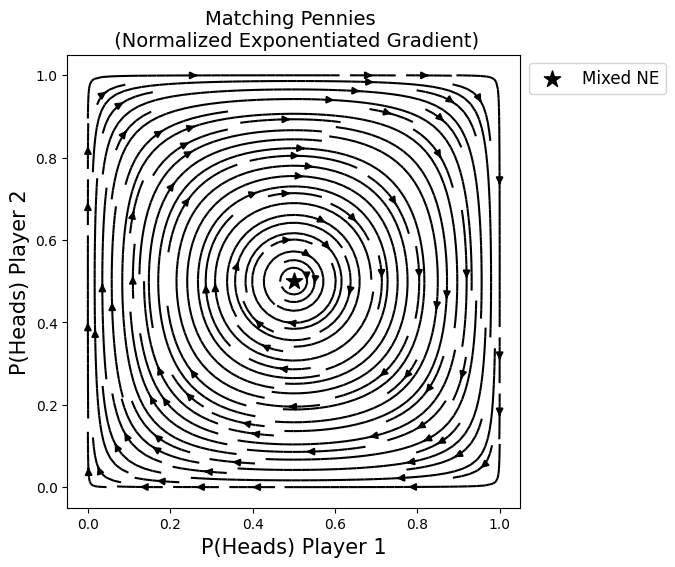
\includegraphics[width=0.5\textwidth]{logos/Pennies1.png}
    \caption{NEG vector field in Matching Pennies}
    \label{fig:Pennies1}
\end{figure}

\begin{figure}[H]
    \centering
    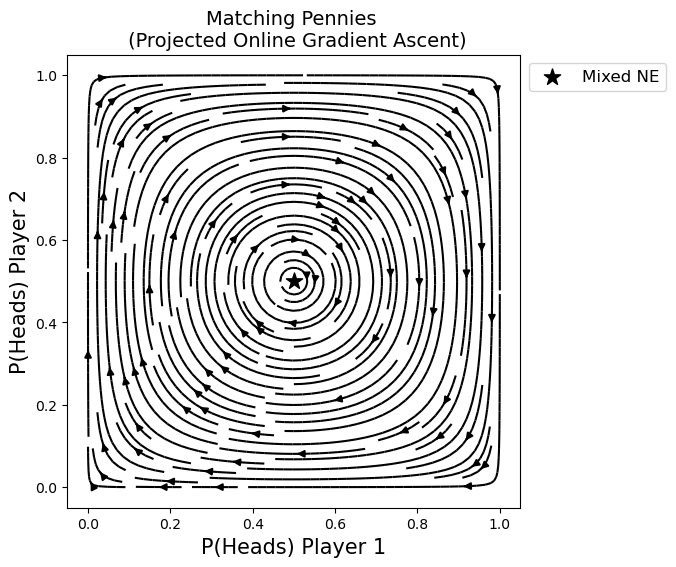
\includegraphics[width=0.5\textwidth]{logos/Pennies2.png}
    \caption{OGALP vector field in Matching Pennies}
    \label{fig:Pennies2}
\end{figure}

Interestingly, the empirical frequency of play, however, ultimately converges to the unique MNE. That happened independently from the initial strategies of the players. The amplitude of of cycles dampens over time as in figure \ref{fig:Pennies3}.

\begin{figure}[H]
    \centering
    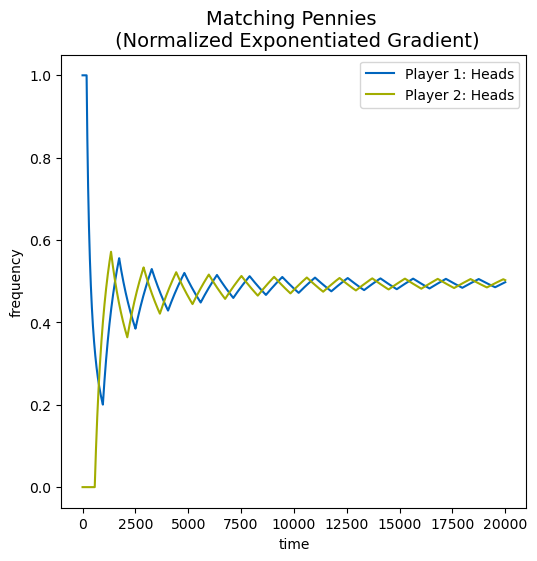
\includegraphics[width=0.5\textwidth]{logos/Pennies3.png}
    \caption{NEG empirical frequency of play in Matching Pennies}
    \label{fig:Pennies3}
\end{figure}


\subsection{Rock Paper Scissors}\label{subsection:rockPaperScissors}

One might think the convergence of empirical frequencies to the game's MNE is an artifact of its simple 2x2 structure, but I found similar behavior in Rock Paper Scissors, another constant-sum game.

\begin{table}[H]\centering
\setlength{\extrarowheight}{2pt}
\begin{tabular}{cc|c|c|c|}
  & \multicolumn{1}{c}{} & \multicolumn{1}{c}{$Rock$}  & \multicolumn{1}{c}{$Paper$}  & \multicolumn{1}{c}{$Scissors$} \\\cline{3-5}
            & $Rock$ & $0,0$ & $-1,1$ & $1,-1$ \\ \cline{3-5}
            & $Paper$ & $1,-1$ & $0,0$ & $-1,1$ \\\cline{3-5}
            & $Scissors$ & $-1,1$ & $1,-1$ & $0,0$ \\\cline{3-5}
\end{tabular}\caption{\label{tab:payoffRPS}payoff matrix Rock Paper Scissors}
\end{table}

The only \textit{Nash equilibrium} that exists is the following \textit{fully mixed} NE

\begin{equation*}
    x_{i}^{*} = (1/3,1/3,1/3) \qquad \forall \quad i \in \mathcal{N}
\end{equation*}

After roughly $50$ timesteps, both algorithms exhibit finite out-of-sync cyclic behavior as shown in figure \ref{fig:RPS2}. The players essentially chase one another. Note that the initial strategies are set randomly. 

\begin{figure}[H]
    \centering
    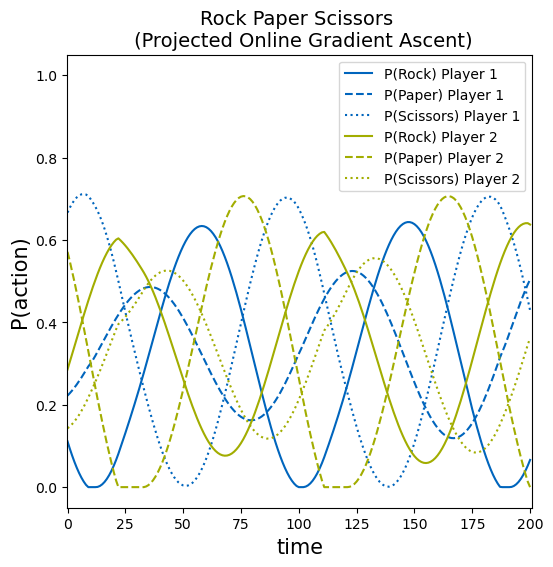
\includegraphics[width=0.5\textwidth]{logos/RPS2.png}
    \caption{OGALP weights in Rock Paper Scissors}
    \label{fig:RPS2}
\end{figure}


Again, the empirical frequencies, on the other hand, converge to the game's unique MNE as in figure \ref{fig:RPS3}

\begin{figure}[H]
    \centering
    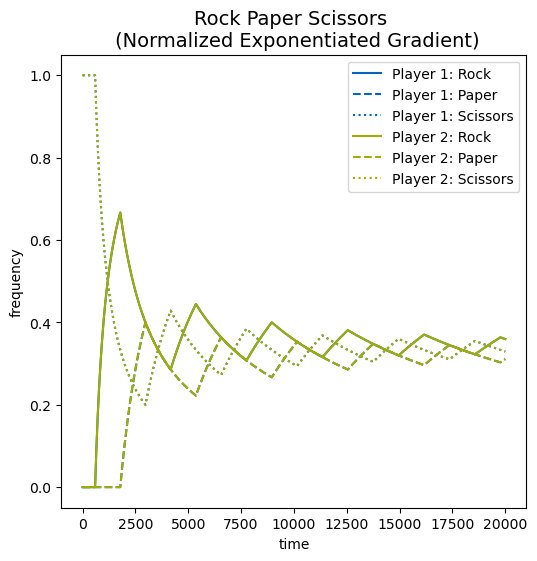
\includegraphics[width=0.5\textwidth]{logos/RPS3.png}
    \caption{NEG empirical frequency of play in Rock Paper Scissors}
    \label{fig:RPS3}
\end{figure}


\subsection{Shapley Game}\label{subsection:shapleyGame}

The Shapley Game resembles that of Rock Paper Scissors. But Shapley is not constant-sum but general-sum.  

\begin{table}[H]\centering
\setlength{\extrarowheight}{2pt}
\begin{tabular}{cc|c|c|c|}
  & \multicolumn{1}{c}{} & \multicolumn{1}{c}{$L$}  & \multicolumn{1}{c}{$C$}  & \multicolumn{1}{c}{$R$} \\\cline{3-5}
            & $T$ & $1,0$ & $0,1$ & $0,0$ \\ \cline{3-5}
            & $M$ & $0,0$ & $1,0$ & $0,1$ \\\cline{3-5}
            & $B$ & $0,1$ & $0,0$ & $1,0$ \\\cline{3-5}
\end{tabular}\caption{\label{tab:payoffShapley}payoff matrix Shapley Game}
\end{table}

The game's unique NE is the same \textit{fully mixed Nash equilibrium} as in Rock Paper Scissors

\begin{equation*}
    x_{i}^{*} = (1/3,1/3,1/3) \qquad \forall \quad i \in \mathcal{N}
\end{equation*}

In this case, both NEG and OGALP, are non convergent neither in weights nor in frequencies. Again the weights cycle through the space of possible strategies but this time the cycles grow exponentially, see figure \ref{fig:Shapley1}. As far as frequencies are concerned the amplitudes of the cycles do not dampen over time (Fig. \ref{fig:Shapley2}) as it did in Matching Pennies or Rock Paper Scissors. They rather cycle exponentially again. Similar results are shown in \cite{jafari}. They suggest that the convergence of frequencies to the game's MNE is because of its constant sum structure. In general sum games, like the Shapley Game, \textit{no regrets} dynamics fail to converge. The same behaviour was found for \textit{fictitious play}, a simple \textit{best response} dynamic that is not a \textit{no regret} algorithm \cite{jafari}.

\begin{figure}[H]
    \centering
    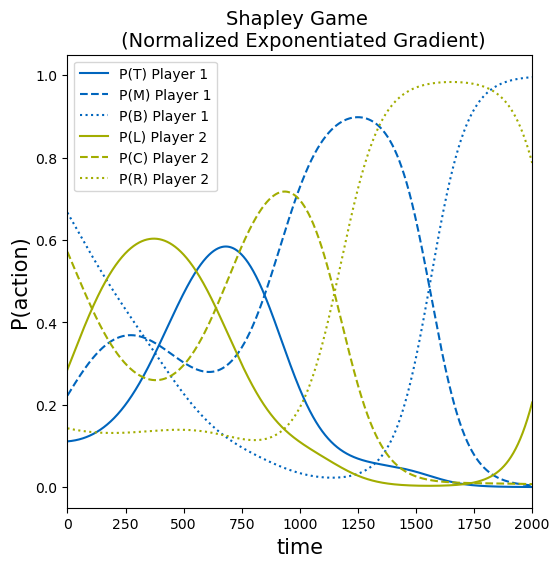
\includegraphics[width=0.5\textwidth]{logos/Shapley1.png}
    \caption{NEG weights in the Shapley Game}
    \label{fig:Shapley1}
\end{figure}

\begin{figure}[H]
    \centering
    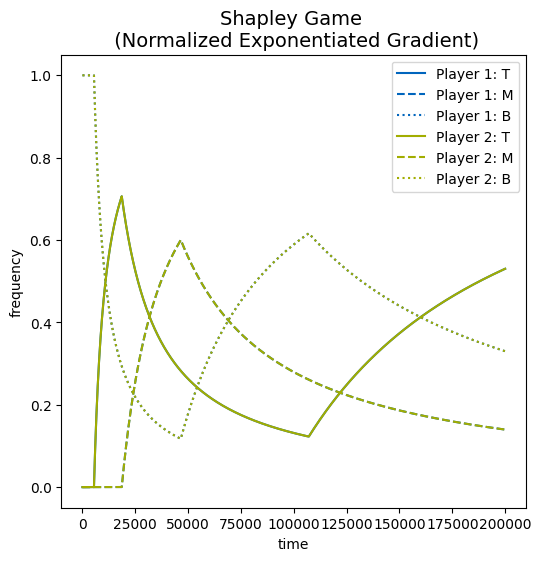
\includegraphics[width=0.5\textwidth]{logos/Shapley2.png}
    \caption{NEG empirical frequency of play in the Shapley Game}
    \label{fig:Shapley2}
\end{figure}



\section{Unique Pure Nash Equilibrium}\label{section:uniquePureNashEquilibrium}

\subsection{Prisoner's Dilemma}\label{subsection:prisonersDilemma}

The next game I would like to address is the famous Prisoner's Dilemma. The game works as follows. Two bank robbers have been arrested. They are separated from each other and both can choose either to stay silent or to betray the other one by admitting the crime. When both stay silent, both are sent to prison for only one year. When both betray they go to jail for 2 years each. However, if one stays silent while the other betrays the one that stayed silent goes is sent to prison for 3 years while the other one is set free, see table \ref{tab:payoffPrisoners}.

\begin{table}[H]\centering
\setlength{\extrarowheight}{2pt}
\begin{tabular}{cc|c|c|}
  & \multicolumn{1}{c}{} & \multicolumn{1}{c}{$Silent$}  & \multicolumn{1}{c}{$Betray$} \\\cline{3-4}
  & $Silent$ & $-1,-1$ & $-3,0$ \\\cline{3-4}
  & $Betray$ & $0,-3$ & $-2,-2$ \\\cline{3-4}
\end{tabular}\caption{\label{tab:payoffPrisoners}payoff matrix Prisoner's Dilemma}
\end{table}

The only \textit{Nash equilibrium} is when both players always choose \textit{Betray}. So there is no \textit{fully mixed Nash equilibrium} but only one \textit{pure Nash equilibrium}. 

\begin{equation*}
    x^{*} = (Betray,Betray) \qquad \textit{strict }\text{PNE}
\end{equation*}

Note that the PNE is also \textit{strict}. Any unilateral deviation from the PNE would lead to a reduction in payoff. For instance, if the \textit{row player} knows that the \textit{column player}  chooses \textit{Betray} then deviating from \textit{Betray} would decrease the \textit{row player's} payoff, from $-2$ to $-3$. As the game is symmetric the same holds for the \textit{column player}. \\

The blue region in figure \ref{fig:Prisoners2} indicates strategies that are \textit{stable} with respect to the PNE in a sense of definition \ref{def:stability}. As we can see the PNE is \textit{globally stable}. As stated in proposition \ref{prop:globalConvergence} \textit{no-regret} dynamics converge globally to the \textit{globally stable equilibrium}. As the vector field in the same figure \ref{fig:Prisoners2} suggests, NEG indeed converges globally to the games's unique PNE. We have the same result for OGDLP, see figure \ref{fig:Prisoners3}.

\begin{figure}[H]
    \centering
    \captionsetup{justification=centering}
    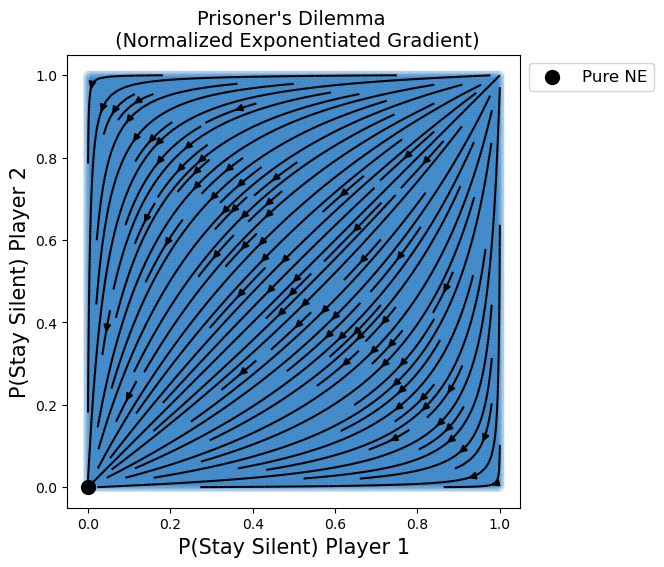
\includegraphics[width=0.5\textwidth]{logos/Prisoners2.png}
    \caption{NEG vector field in Prisoner's Dilemma. Stable region with respect to the PNE is colored in blue}
    \label{fig:Prisoners2}
\end{figure}

\begin{figure}[H]
    \centering
    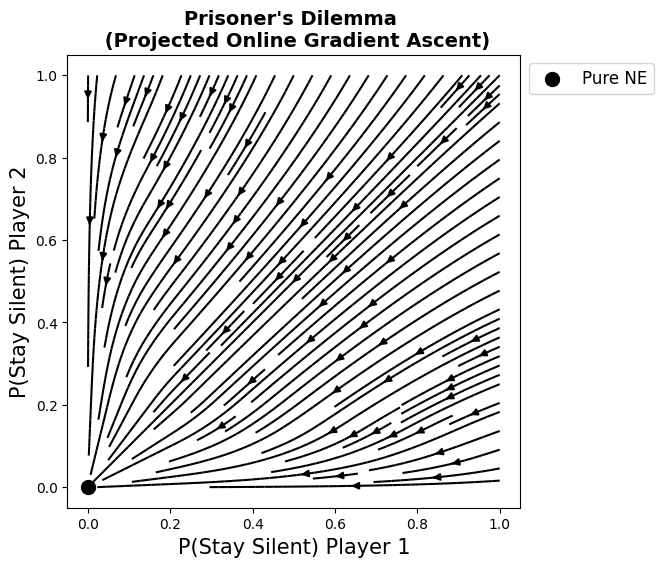
\includegraphics[width=0.5\textwidth]{logos/Prisoners3.png}
    \caption{OGDLP vector field in Prisoner's Dilemma}
    \label{fig:Prisoners3}
\end{figure}

\section{Mixed and Pure Nash Equilibria}\label{section:MixedandPureNashEquilibria}

\subsection{Battle Of Sexes}\label{subsection:battleOfSexes}

Image a couple of two persons with different interests. One would prefer to watch a boxing fight, say the \textit{row player}, and the other one prefers to go to a ballet, the \textit{column player}. But they would rather spend time together than choosing different events. There is no communication between both. The payoff is set accordingly as in table \ref{tab:payoffBattleOfSexes}.

\begin{table}[H]\centering
\setlength{\extrarowheight}{2pt}
\begin{tabular}{cc|c|c|}
  & \multicolumn{1}{c}{} & \multicolumn{1}{c}{$Fight$}  & \multicolumn{1}{c}{$Ballet$} \\\cline{3-4}
  & $Fight$ & $3,2$ & $0,0$ \\\cline{3-4}
  & $Ballet$ & $0,0$ & $2,3$ \\\cline{3-4}
\end{tabular}\caption{\label{tab:payoffBattleOfSexes}payoff matrix Battle of Sexes}
\end{table}

There are two quite obvious \textit{pure Nash equilibria}. One where both choose \textit{Fight}, and one where both choose \textit{Ballet}. But there is also a \textit{fully mixed Nash equilibrium}, i.e when both players randomize over the actions. In particular the \textit{row player} should choose \textit{Fight} with probability $2/3$ and \textit{Ballet} with $1/3$ and the \textit{column player} should choose \textit{Fight} with $1/3$ and \textit{Ballet} with $2/3$. In formulas we have the following \textit{Nash equilibria}

\begin{description}\centering
    \item $x^{*} = (Fight,Fight) \qquad \textit{strict }\text{PNE}$
    \item $x^{*} = (Betray,Betray) \qquad \textit{strict }\text{PNE}$
    \item $x_{1}^* = (2/3,1/3) \qquad x_{2}^* = (1/3,2/3) \qquad \text{MNE}$
\end{description}

Note that again both PNEs are \textit{strict} in a sense of definition \ref{def:strictNE}. Neither the \textit{row player} nor the \textit{column player} can unilaterally deviate from an PNE without reducing its payoff. According to proposition \ref{prop:StrictStableEquivalent} that means both PNE are also \textit{stable} states as defined in \ref{def:stability}. Then both PNEs must also be locally attracting (proposition \ref{prop:localConvergence}). And indeed, as shown in figure \ref{fig:BattleOfSexes5}, the NEG algorithm converges locally to the corresponding PNE. Notice how the stable regions of the PNEs intersect. 

\begin{figure}[H]
    \centering
    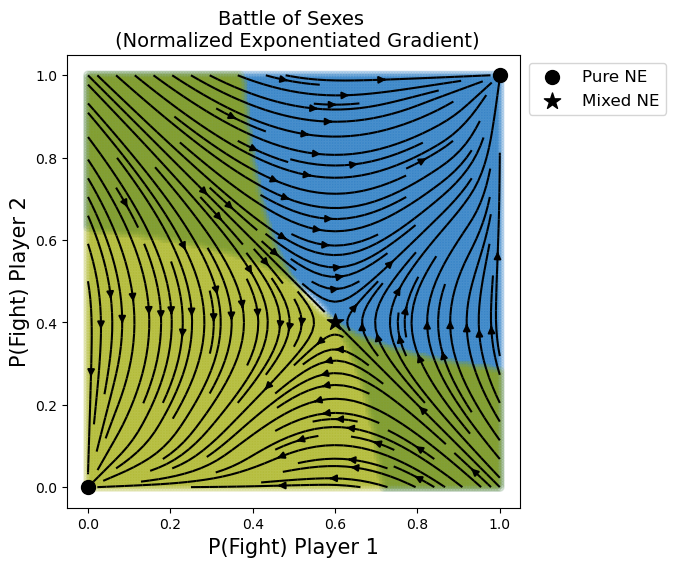
\includegraphics[width=0.5\textwidth]{logos/BattleOfSexes5.png}
    \caption{NEG vector field in Battle of Sexes with stable regions for both PNEs}
    \label{fig:BattleOfSexes5}
\end{figure}

For clarification I have highlighted only the stable region with respect to the PNE \textit{(Fight,Fight)} in figure \ref{fig:BattleOfSexes2}. Also notice that not all points in the stable region converge to the corresponding PNE. In this game, for instance, all initial point above the diagonal between \textit{(Fight,Ballet)} and \textit{(Ballet,Fight)} converge to the PNE \textit{(Fight,Fight)} and all point below converge to the PNE \textit{(Ballet,Ballet)}. 

\begin{figure}[H]
    \centering
    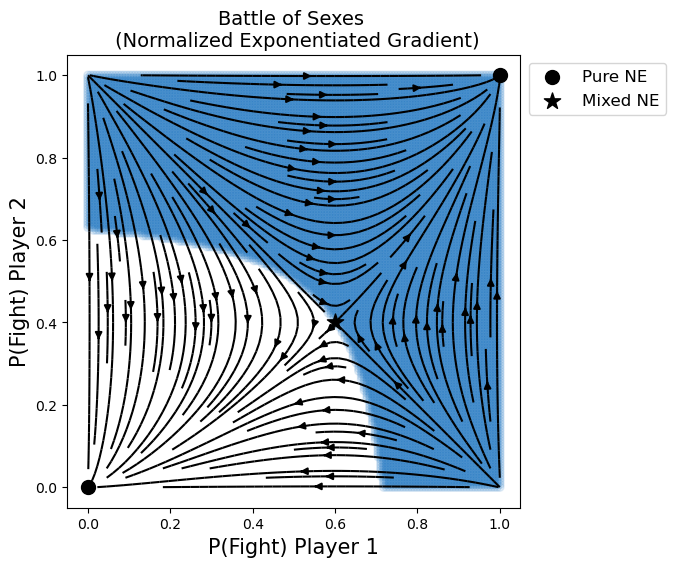
\includegraphics[width=0.5\textwidth]{logos/BattleOfSexes2.png}
    \caption{NEG vector field in Battle of Sexes with stable regions for the PNE \textit{(Fight,Fight)}}
    \label{fig:BattleOfSexes2}
\end{figure}

The question might raise whether the MNE can be \textit{stable} as well. Even though there is a stable region for the MNE as depicted in \ref{fig:BattleOfSexes3}, we cannot find a neighborhood for the MNE such that the inequality of the stability definition (\ref{def:stability}) holds. Intuitively, no matter how far we zoom in to the MNE we cannot draw a circle around it such that all points within the circle are blue as illustrated in figure \ref{fig:BattleOfSexes4}. Therefore except from the perfect diagonal between \textit{(Fight,Ballet)} and \textit{(Ballet,Fight)} the algorithms never converges towards the MNE. That is align with proposition \ref{prop:noInteriorStable} that no interior point can be \textit{stable} under FoReL.  

\begin{figure}[H]
    \centering
    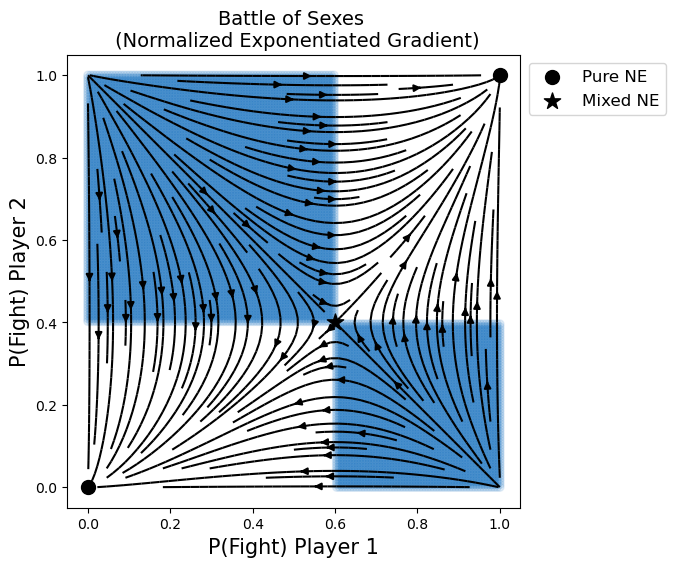
\includegraphics[width=0.5\textwidth]{logos/BattleOfSexes3.png}
    \caption{Stable region for MNE in Battle of Sexes}
    \label{fig:BattleOfSexes3}
\end{figure}

\begin{figure}[H]
    \centering
    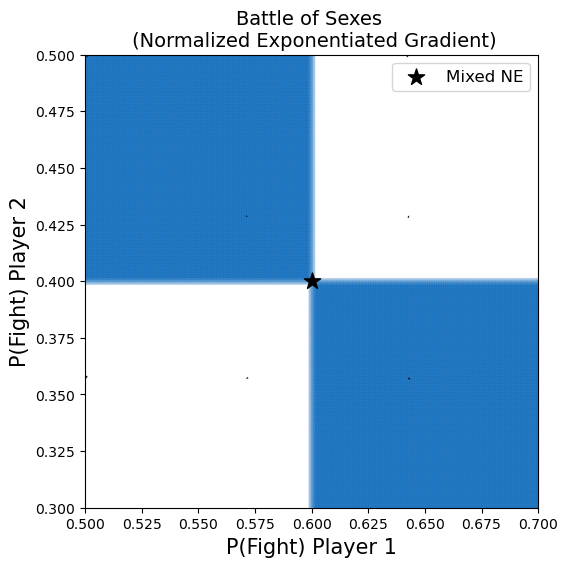
\includegraphics[width=0.5\textwidth]{logos/BattleOfSexes4.png}
    \caption{Zoomed in to the MNE in Battle of Sexes}
    \label{fig:BattleOfSexes4}
\end{figure}


\subsection{Intersection Game}\label{subsection:intersectionGame}

Lets revisit the intersection game from subsection \ref{subsection:CEandCCE}. The game involves two car drivers that need to cross an intersection without a crash. They can either \textit{Stop} or \textit{Go}. The driver's payoff is straight forward as in table \ref{tab:payoffIntersection}. 

\begin{table}[H]\centering
\setlength{\extrarowheight}{2pt}
\begin{tabular}{cc|c|c|}
  & \multicolumn{1}{c}{} & \multicolumn{1}{c}{$Stop$}  & \multicolumn{1}{c}{$Go$} \\\cline{3-4}
  & $Stop$ & $0,0$ & $0,1$ \\\cline{3-4}
  & $Go$ & $1,0$ & $-100,-100$ \\\cline{3-4}
\end{tabular}\caption{\label{tab:payoffIntersection}payoff matrix Intersection Game}
\end{table}

Similar to the Battle of Sexes the game has two \textit{pure Nash equilibria}, namely \textit{(Stop, Stop)} and \textit{(Go,Go)}, and a single \textit{mixed Nash equilibrium} where both drivers choose to \textit{Stop} with probability $100/101$ and \textit{Go} with probability $1/101$. To sum up we have the following \textit{Nash equilibria}.

\begin{description}\centering
    \item $x^{*} = (Go,Go) \qquad \textit{strict }\text{PNE}$
    \item $x^{*} = (Stop,Stop) \qquad \textit{strict }\text{PNE}$
    \item $x_{1}^* = x_{2}^* = (100/101,1/101) \qquad \text{MNE}$
\end{description}

Again it is easy to check that both PNEs are also \textit{strict} and therefore \textit{stable} states (proposition \ref{prop:StrictStableEquivalent}). I have colored the \textit{stable} regions for both PNEs. We can see that both PNEs are indeed \textit{locally stable} states. Just like stated in proposition \ref{prop:localConvergence} our \textit{no-regret} algorithms therefore need to locally converge to the PNEs. In fact both algorithms converge to the PNE that is the "closest" one from the initial strategy just like in Battle of Sexes, see figure \ref{fig:Intersection4}. Note that the MNE denoted by the star is indeed a \textit{fully mixed} NE even though it looks like a PNE.

\begin{figure}[H]
    \centering
    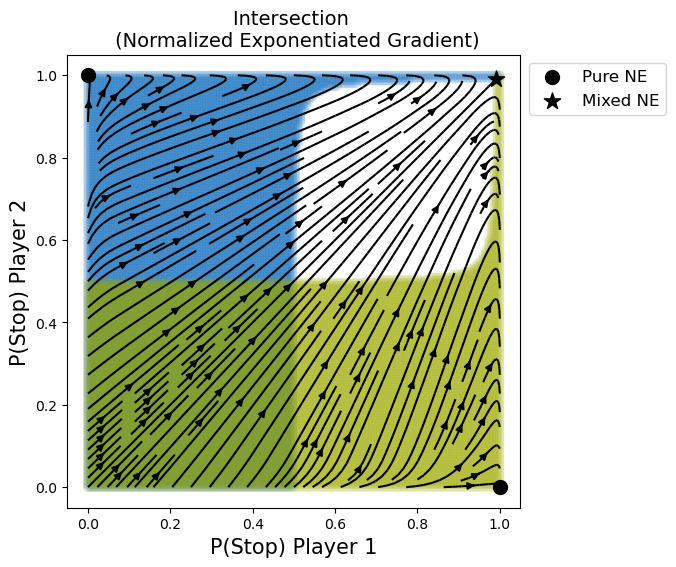
\includegraphics[width=0.5\textwidth]{logos/Intersection4.png}
    \caption{NEG vector field in the Intersection game with stable regions colored}
    \label{fig:Intersection4}
\end{figure}

Figure \ref{fig:Intersection4} might be misleading as is seems like the algorithm converges to the MNE. Even though the MNE seems to be attracting, both algorithms eventually converge to an PNE for all initial strategies except from the perfect diagonal. I have plotted a single trajectory in figure \ref{fig:Intersection5} to clarify that. 

\begin{figure}[H]
    \centering
    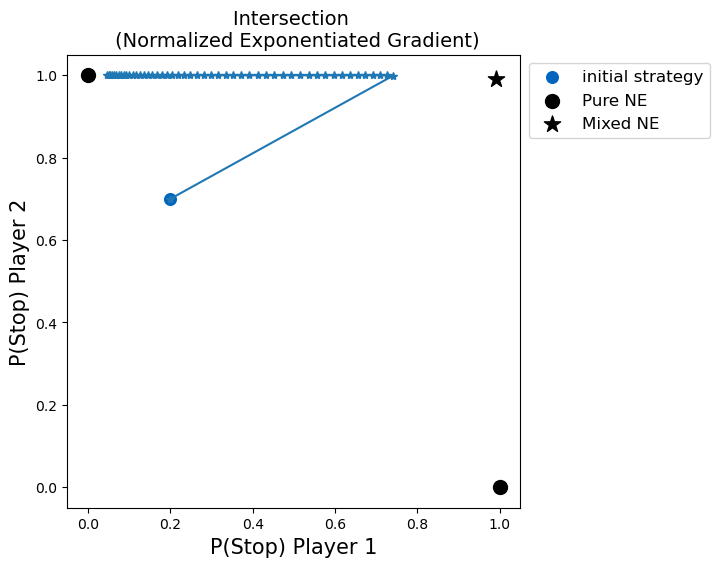
\includegraphics[width=0.5\textwidth]{logos/Intersection5.png}
    \caption{NEG single trajectory for the initial strategy $x_{1}^{0} = (0.2,0.8)$, $x_{1}^{0} = (0.7,0.3)$}
    \label{fig:Intersection5}
\end{figure}

Just like in Battle of Sexes we cannot find a neighborhood for the MNE such that the equation of the stability definition \ref{def:stability} is fulfilled. As we zoom in to the MNE again we cannot draw a circle around the MNE such that all points within the circle are colored, as illustrated in figure \ref{fig:Intersection6}. The same observations could be made for OGDLP. 

\begin{figure}[H]
    \centering
    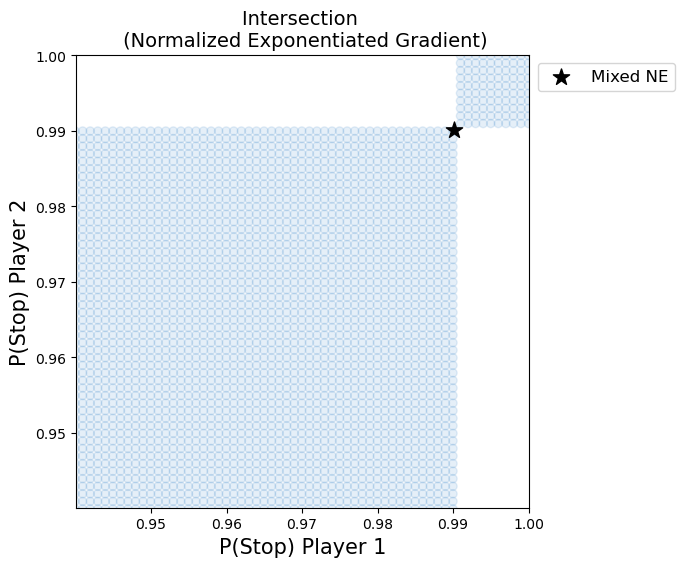
\includegraphics[width=0.5\textwidth]{logos/Intersection6.png}
    \caption{Zoomed in to the MNE in the Intersection Game}
    \label{fig:Intersection6}
\end{figure}


\subsection{Coordination Game}\label{subsection:coordinationGame}

The behaviour of the Coordination game under \textit{no-regret} dynamics has already been studied in \cite{jafari} but other \textit{no-regret} algorithms than NEG and OGDLP were used. As the name suggests, both player aim to cooperate, see table \ref{tab:payoffCoordination3x3}. 

\begin{table}[H]\centering
\setlength{\extrarowheight}{2pt}
\begin{tabular}{cc|c|c|c|}
  & \multicolumn{1}{c}{} & \multicolumn{1}{c}{$L$}  & \multicolumn{1}{c}{$C$}  & \multicolumn{1}{c}{$R$} \\\cline{3-5}
            & $T$ & $3,3$ & $0,0$ & $0,0$ \\ \cline{3-5}
            & $M$ & $0,0$ & $2,2$ & $0,0$ \\\cline{3-5}
            & $B$ & $0,0$ & $0,0$ & $1,1$ \\\cline{3-5}
\end{tabular}\caption{\label{tab:payoffCoordination3x3}payoff matrix Coordination Game}
\end{table}

There are three \textit{pure Nash equilibria} and multiple \textit{fully mixed Nash equilibria}. As we have seen in the previous examples \textit{fully mixed Nash equilibria} are not \textit{stable} therefore not learnable under \textit{no-regret} dynamics. For that reason we will neglect MNEs from now on. Lets consider the following three PNEs.

\begin{description}\centering
    \item $x^{*} = (T,L) \qquad \textit{strict }\text{PNE}$
    \item $x^{*} = (M,C) \qquad \textit{strict }\text{PNE}$
    \item $x^{*} = (B,R) \qquad \textit{strict }\text{PNE}$
\end{description}

Obviously all of them are \textit{strict} PNEs as any unilateral deviation from an PNE results in a decrease in payoff. Note that \textit{(B,R)} is \textit{pareto dominated} by \textit{(M,C)} which is once again \textit{pareto dominated} by \textit{(T,L)}, so \textit{(T,L)} is \textit{pareto optimal}. \\

One might assume that for any general-sum game that is not constant-sum \textit{no-regret} algorithms do not converge as we observed in the Shapley Game in subsection \ref{subsection:shapleyGame}. In the Coordination game however I found convergence to one of the above PNEs for all initial strategies. I have randomized the players' initail strategies and actually most of the time both algorithms converged to the \textit{pareto optimal} PNE \textit{(T,L)} (see an example in figure \ref{fig:Coordination3x3-1}). 

\begin{figure}[H]
    \centering
    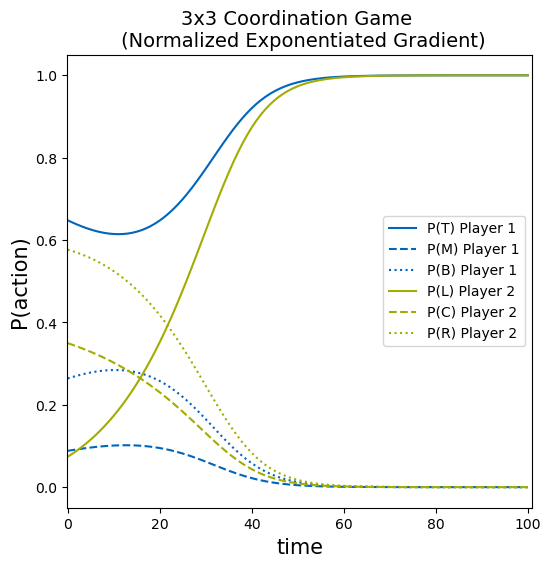
\includegraphics[width=0.5\textwidth]{logos/Coordination3x3-1.png}
    \caption{NEG convergence to the PNE \textit{(T,L)}}
    \label{fig:Coordination3x3-1}
\end{figure}

Less often I found convergence to the PNE \textit{(M,C)} (see figure \ref{fig:Coordination3x3-2}) and even less often to the PNE \textit{(B,R)} (see figure \ref{fig:Coordination3x3-3}). Unfortunately I haven't found a pattern for which initial strategy the algorithms converge to a specific PNE but the fact that most of the time it converges to \textit{(T,L)} might probably have something to do with its \textit{pareto dominance}. 

\begin{figure}[H]
    \centering
    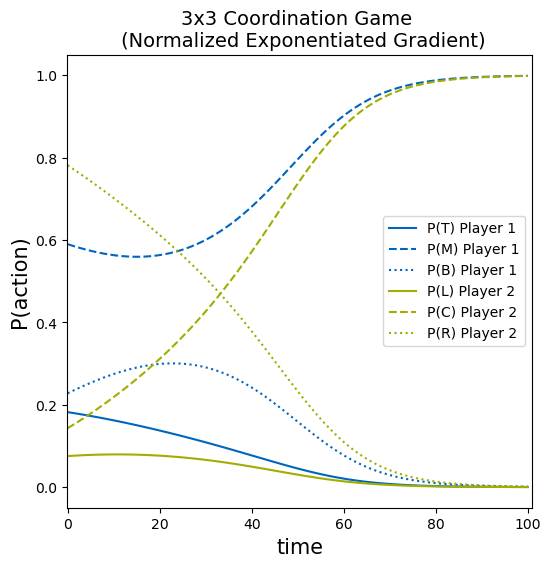
\includegraphics[width=0.5\textwidth]{logos/Coordination3x3-2.png}
    \caption{NEG convergence to the PNE \textit{(M,C)}}
    \label{fig:Coordination3x3-2}
\end{figure}

\begin{figure}[H]
    \centering
    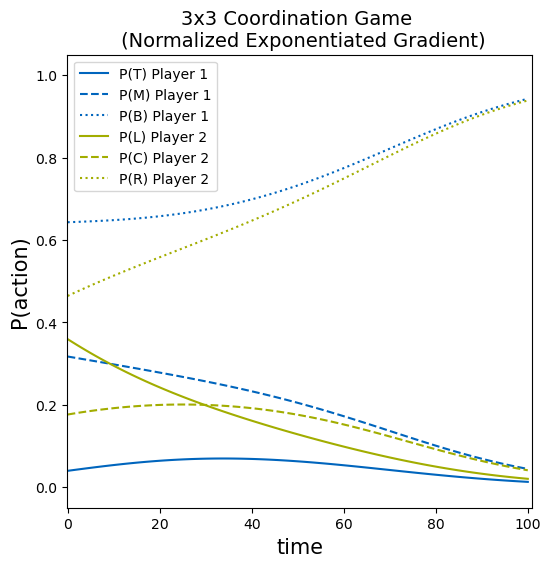
\includegraphics[width=0.5\textwidth]{logos/Coordination3x3-3.png}
    \caption{NEG convergence to the PNE \textit{(B,R)}}
    \label{fig:Coordination3x3-3}
\end{figure}

The reason why both algorithms converge to \textit{Nash equilibria} in the Coordination game and diverge in the Shapley Game is because there exists no \textit{strict} NE in the Shapley Game. As we have concluded in chapter \ref{chapter:literatureReview} only \textit{strict} NE survive under \textit{no-regret} dynamics which means in games where no \textit{strict} NE exists we need to expect that the induced sequence of play diverges, as it did in the Shapley game. Note that empirical frequency of play might still converge even though no \textit{strict} NE exists as we observed in the constant-sum games Matching Pennies and Rock Paper Scissors. 


\section{Weak Nash Equilibria}\label{section:WeakNashEquilibria}

\subsection{2x2}\label{subsection:2x2}

\begin{table}[H]\centering
\setlength{\extrarowheight}{2pt}
\begin{tabular}{cc|c|c|}
  & \multicolumn{1}{c}{} & \multicolumn{1}{c}{$H$}  & \multicolumn{1}{c}{$T$} \\\cline{3-4}
  & $H$ & $2,3$ & $1,2$ \\\cline{3-4}
  & $T$ & $1,2$ & $2,2$ \\\cline{3-4}
\end{tabular}\caption{\label{tab:payoffStrictAndWeak2x2}payoff matrix Strict and Weak Nash Equilibria 2x2}
\end{table}

\begin{itemize}
    \item quickly explain the game and why there is both a strict and a weak NE according to \ref{section:equilibriaConcepts}
    \item Note that the plots are misleading as the trajectory stays within the simplex but for some initial points
    it diverges towards the "left wall". 
    \item Still both algorithms never converge towards the weak NE
    \item When getting numerically close to the weak NE it get unstable, i.e variational stability is positive
    \item Unclear how to interpret \cite{flokas} Flokas Theorem 2 
    \item The weak NE seems to disrupt the convergence to the strict NE. 
    \item As the strictly NE is locally stable it is locally attracting (but definitely not globally)
\end{itemize}

\begin{figure}
    \centering
    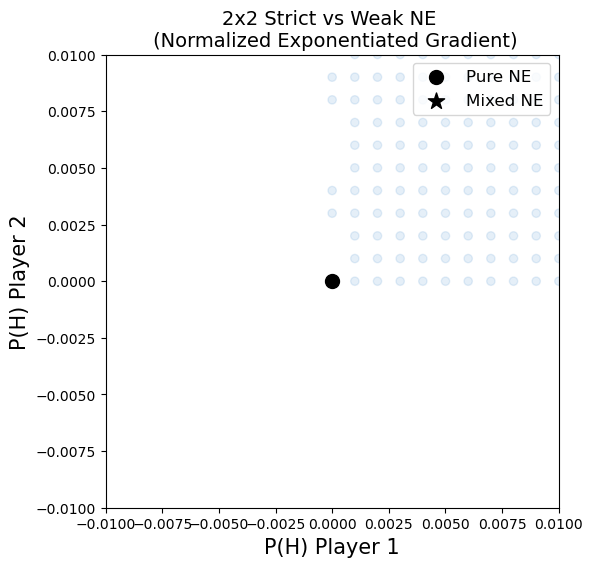
\includegraphics[width=0.5\textwidth]{logos/Weak1.png}
    \caption{...}
    \label{fig:Weak1}
\end{figure}

\begin{figure}
    \centering
    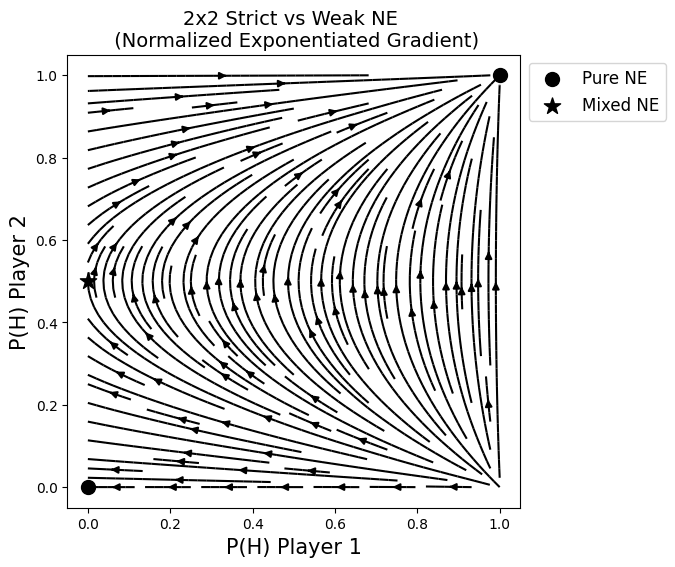
\includegraphics[width=0.5\textwidth]{logos/Weak2.png}
    \caption{...}
    \label{fig:Weak2}
\end{figure}

\begin{figure}
    \centering
    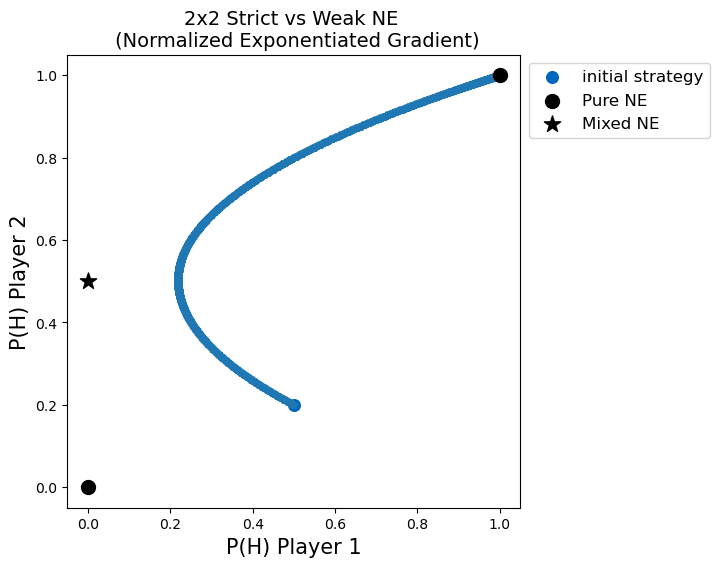
\includegraphics[width=0.5\textwidth]{logos/Weak3.png}
    \caption{...}
    \label{fig:Weak3}
\end{figure}

\begin{figure}
    \centering
    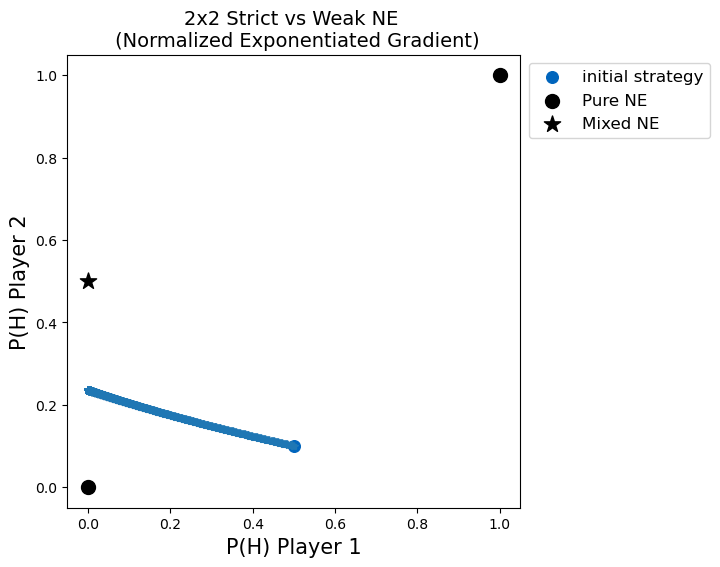
\includegraphics[width=0.5\textwidth]{logos/Weak4.png}
    \caption{...}
    \label{fig:Weak4}
\end{figure}

\begin{figure}
    \centering
    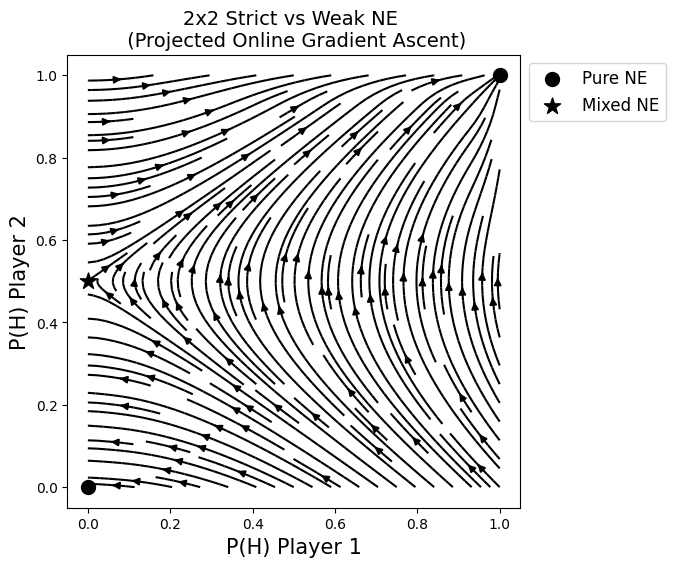
\includegraphics[width=0.5\textwidth]{logos/Weak5.png}
    \caption{...}
    \label{fig:Weak5}
\end{figure}

\begin{figure}
    \centering
    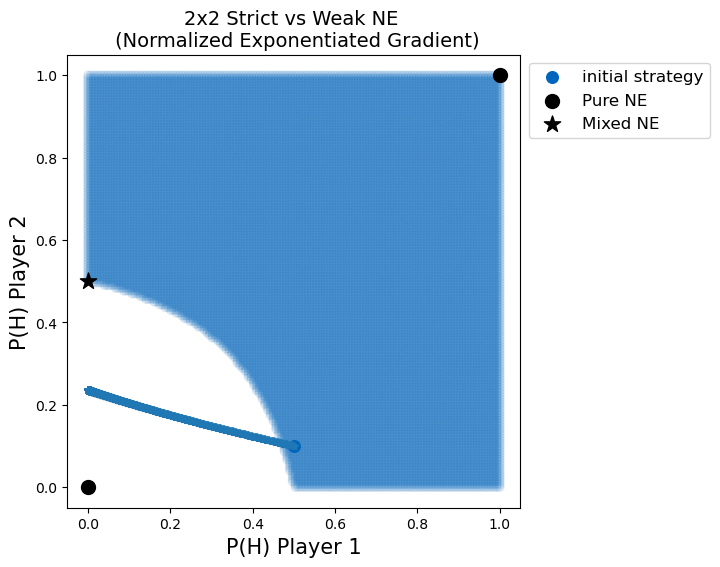
\includegraphics[width=0.5\textwidth]{logos/Weak6.png}
    \caption{...}
    \label{fig:Weak6}
\end{figure}


\subsection{3x3}\label{subsection:3x3}

\begin{table}\centering
\setlength{\extrarowheight}{2pt}
\begin{tabular}{cc|c|c|c|}
  & \multicolumn{1}{c}{} & \multicolumn{1}{c}{$A$}  & \multicolumn{1}{c}{$B$}  & \multicolumn{1}{c}{$C$} \\\cline{3-5}
            & $X$ & $2,3$ & $1,2$ & $1,1$ \\ \cline{3-5}
            & $Y$ & $1,1$ & $2,1$ & $3,2$ \\\cline{3-5}
            & $Z$ & $1,2$ & $2,2$ & $2,1$ \\\cline{3-5}
\end{tabular}\caption{\label{tab:payoffStrictAndWeak3x3}payoff matrix Strict and Weak Nash Equilibria 3x3}
\end{table}

\begin{itemize}
    \item Always converging towards Strict PNE (X,A), (Y,C)
    \item Never converging to the Weak PNE (Y,B)
\end{itemize}

\begin{figure}
    \centering
    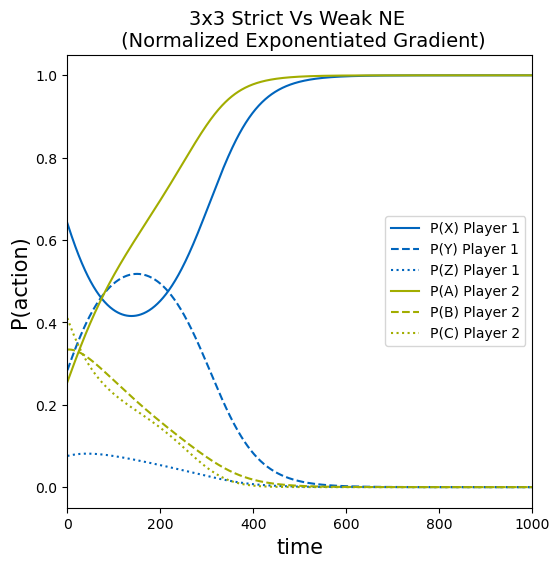
\includegraphics[width=0.5\textwidth]{logos/Weak3x3-1.png}
    \caption{...}
    \label{fig:Weak3x3-1}
\end{figure}

\begin{figure}
    \centering
    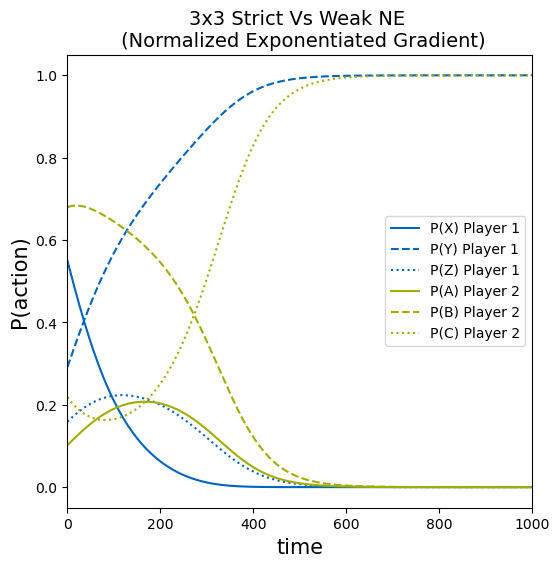
\includegraphics[width=0.5\textwidth]{logos/Weak3x3-2.png}
    \caption{...}
    \label{fig:Weak3x3-2}
\end{figure}
